\chapter{Alkali-doped nanodroplets}

	In their 1996 paper\citep{Griffin1996} Griffin and Stringari have argued that almost 100\% Bose-Einstein Condensation could be achieved in the low density surface region of superfluid He at $T=0$, as opposed to only about 10\% in the bulk. It is therefore evident that a minimally perturbing probe capable of investigating the surface of a He cluster is very desirable.\\

	It comes as no surprise then that alkali atoms are a very natural choice for exactly these type of studies.  For example, with a solvation parameter of $\lambda=0.729$\citep{Anc95}, Rb will remain bound to the surface of the droplet. Furthermore, they have a simple, well known, absorption spectrum. They introduce only weak perturbations (alkali-helium interaction energies are on the order of 1 cm$^{-1}$ [8]). Moreover, their simple, one-valence electron structure allows for detailed theoretical modelling. Lastly, theoretical calculations [9, 10] and experimental spectra [11-13] of alkali atoms in bulk liquid helium are available for comparison.

	Surprisingly, the study of alkali atoms seeded in highly quantum matrices is relevant to the optimisation of the use of solid hydrogen as a rocket propellant\citep{Carrick1993}.\\
	
	Given that the alkalies are ideal probes to probe the boundary region of the nanodroplets, the $n\mathrm{p}\,^2\mathrm{P}\leftarrow n\mathrm{s}\,^2\mathrm{S}$ transitions of the alkali atoms have attracted much interest from an experimental and theoretical point of view. The spectroscopy of the higher excited states has been thoroughly explored[32-42]. The obtained spectra can be successfully reproduced by a pseudo-diatomic model[9,21], except for the higher excited states, where the model progressively fails due to the limitations imposed by its realm of validity. While the the effect of the excited states on the spectra are now fairly well understood, their influence on the following dynamics is largely unexplored.\\
	
	In this part of the thesis, the results of the real-time dynamics of a single electronically excited rubidium (Rb) atom, residing in the surface dimple of a helium nano-droplet will be presented. The atom will be excited from its ground state 5s$\,^2\Sigma_{1/2}$ to the 5p$\,^2\{\Sigma,\Pi\}$ and 6p$\,^2\{\Sigma,\Pi\}$ manifold. This will be a combined experimental and theoretical study.
	
	\section{Experimental setup}

		\begin{figure}[t]
			\begin{center}
				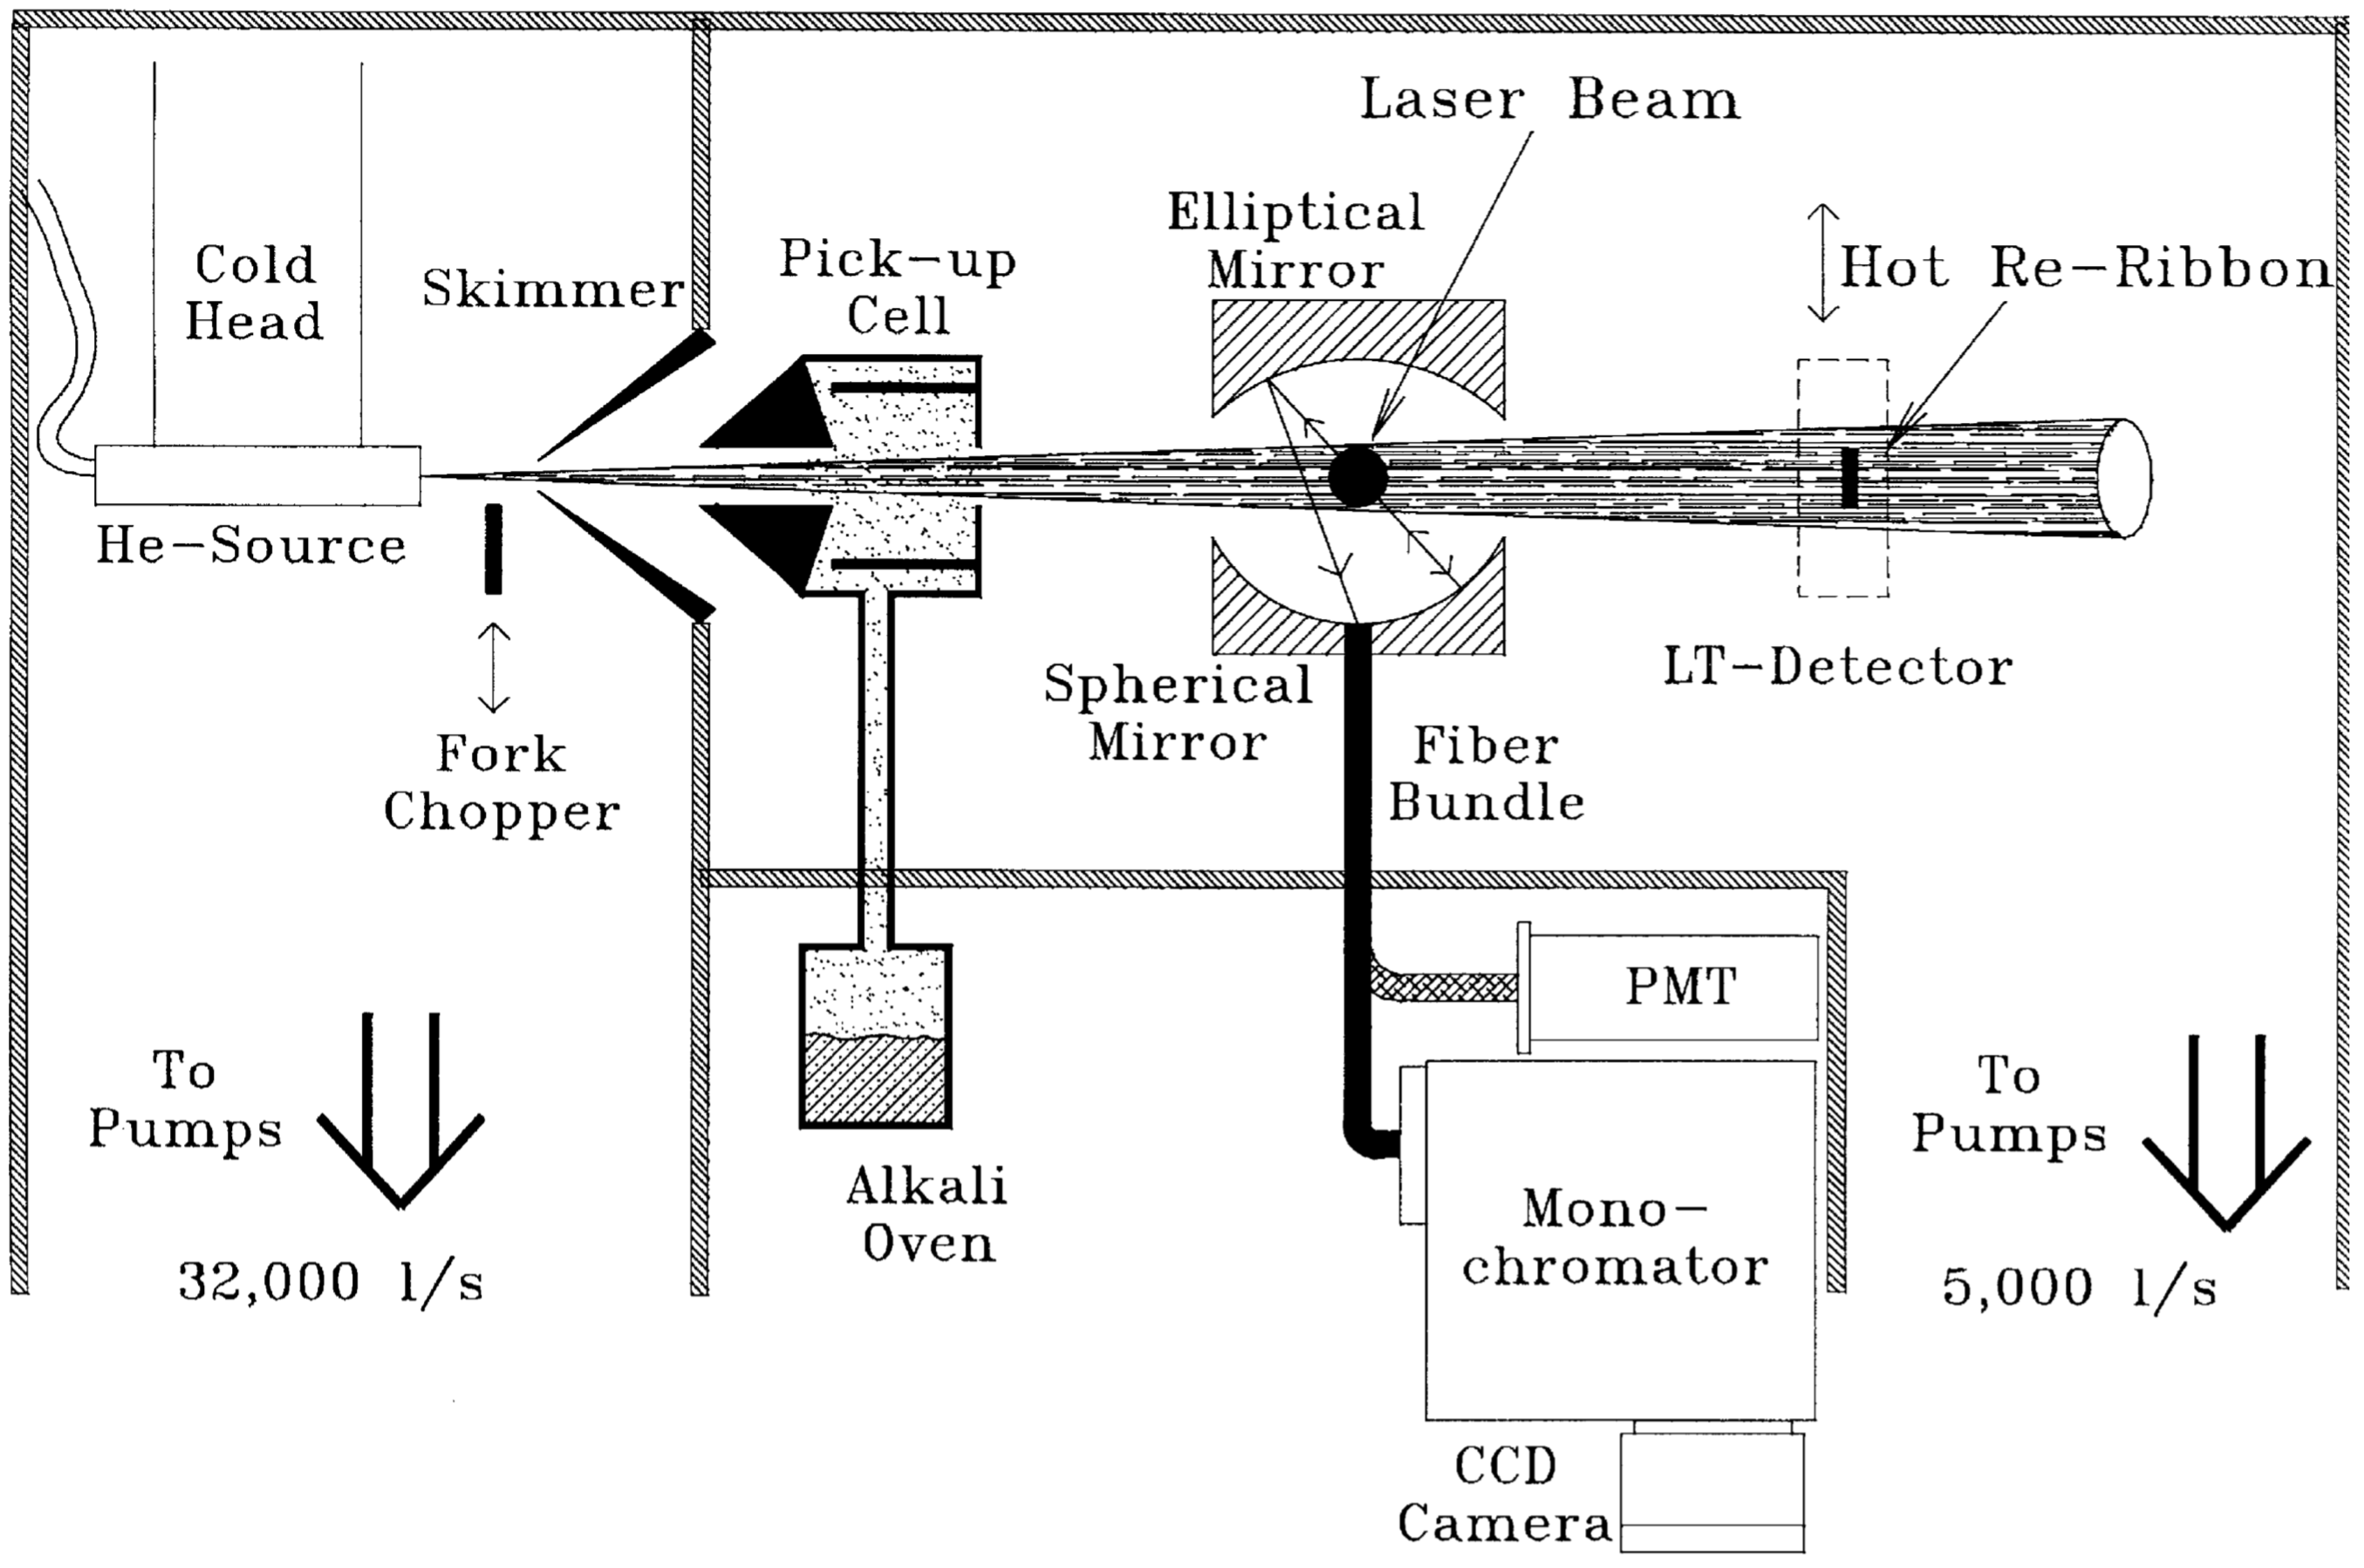
\includegraphics[width=\textwidth]{droplet-beam}
				\caption{Caption}
				\label{fig:droplet-beam}
			\end{center}
		\end{figure}
		
		\lettrine[lines=3,findent=3pt,nindent=0pt]{A}{} beam of large He clusters is produced in a supersonic expansion from a cold nozzle (Fig. \ref{fig:droplet-beam}). The weak He-He binding energy of 7.7 cm$^{-1}$ [22] requires high stagnation pressures and low nozzle temperatures ($T$) for large cluster formation. In our apparatus two CTI cryocoolers are used to establish low temperature conditions (down to 12 K) at the source. The first cooler directly cools the nozzle while the second pre-cools the supplied gas. This is needed because, even for small nozzle diameters (10$\unit{\mu m}$), at stagnation pressures up to 10$^7$ Pa the 1/$\sqrt{T}$ dependence of the gas flux leads to heavy gas loads. The pre-cooling system also provides for gas purification. The high gas throughput is easily handled by a 32000 1/s diffusion pump.
		
		At these low temperatures seeding clusters with a chromophore cannot be achieved by co-expansion and the pick-up seeding method becomes necessary [23]. According to this method, the cluster beam is sent through a scattering cell (located a short distance after the skimmer) in which a variable pressure (10$^{-3}$--10$^{-1}$ Pa) of the chromophore is maintained by connecting it with an alkali reservoir through a heated tube. The temperature of the pick-up cell, (100 K higher than the reservoir), avoids alkali atom distillation and formation of dimers inside the cell. In their path through the cell the larger clusters pick up alkali atoms without being appreciably deflected. Dissipation of the energy of the captured chromophore is likely to occur by evaporation of He atoms from the clusters, the terminal temperature of which rapidly returns to its pre pick-up value ($\approx$0.4 K) [2].
	
		To probe the picked-up alkali atoms we use laser induced fluorescence (LIF) adopting the photon collection optics design described by Hefter and Bergmann in [24]. The intersection point of the laser and cluster beam from which the fluorescence photons are collected is located a few centimetres downstream of the pick-up cell. The light of the probe laser is introduced in the apparatus via a single mode fibre and focusing optics that makes the laser beam diameter at the crossing point approximately the same as the cluster beam diameter ($\approx$2 mm). To sup- press scattered laser light we use a stack of diaphragms forming a baffle of 90 cm length both for the in- and outgoing laser beam. A Woods horn serves as a beam dump. To detect the fluorescence light originating at the point of intersection, the combination of an elliptical and a spherical mirror is used. These two mirrors focus the emitted photons at the entrance of a fibre bundle. The geometrical collection efficiency is 85\% of the 4$\pi$ solid angle centred around the intersection point. After pas- sing through the fibre bundle, the photons reach a photo-multiplier (PMT) for signal detection. The output pulses of the PMT are (after standard amplification and discrimination) stored using two gated counters which follow the cluster beam chopping frequency. Alternatively, a monochromator (GCA / McPherson, EU-700) coupled to a liquid nitrogen cooled CCD detector (Princeton Instruments, LN/CCD 1152 UV) is used for dispersed fluorescence measurements. The absolute frequency of the probe laser is monitored continuously by a home built wave meter with 0.001 cm$^{-1}$ precision. The amount and angular distribution of alkali atoms carried by the clusters can be monitored by means of a Langmuir-Taylor (LT) surface ionisation detector which is located further down- stream and is movable perpendicularly to the cluster beam direction. Since excitation at certain frequencies leads with a significant probability to a desorption of the chromophores from the cluster, we are also able to detect beam depletion spectra. Finally the LT detector provides information on the alkali atom density inside the pick-up cell by measuring the alkali background inside the detection chamber. A computer controls the laser frequency and records the acquisition of photon counts, the actual laser frequency and the parameters for cluster beam and alkali source condition characterisation.


proof is in spectra; not as shifted as in the bulk


finally introduce experiment Vangerov at al 

photo dissociation/ejection all but lowest part of $P_1/2$ excitation

introduce electronic spin relaxation to explain
and Mudrich
